\documentclass[conference]{IEEEtran}
\usepackage[T1]{fontenc}
\usepackage[utf8]{inputenc}
\usepackage[spanish,es-nodecimaldot,es-noindentfirst]{babel}
\usepackage{graphicx}
\usepackage{cite}
\usepackage{array}
\usepackage{xcolor}
\usepackage{colortbl}
\usepackage{multirow}
\usepackage{float}
\usepackage{url}
\usepackage{booktabs}
\usepackage{subcaption}
\usepackage{amssymb}
\usepackage{hyperref}

\hypersetup{
    colorlinks=false,
    pdfborder={0 0 0}
}

\definecolor{colorMalo}{RGB}{170,0,0}
\definecolor{colorBueno}{RGB}{0,110,70}
\definecolor{fecolsogBlue}{RGB}{0,79,159}
\newcommand{\malEjemplo}[1]{\textcolor{colorMalo}{\textit{``#1''}}}
\newcommand{\buenEjemplo}[1]{\textcolor{colorBueno}{\textbf{``#1''}}}

\title{Rediseño de Contenido e Interfaz Inclusiva en la Tienda Online de FECOLSOG}

\author{
\IEEEauthorblockN{Jota Emilio López Ramírez \quad Esmeralda Rivas Guzmán}
\IEEEauthorblockA{Universidad del Valle\\
Ingeniería de Sistemas\\
Tuluá, Colombia}
}

\begin{document}
\maketitle

\begin{abstract}
Este artículo presenta el proceso y los resultados del rediseño de contenido e interfaz de la tienda en línea de la Federación Colombiana de Obstetricia y Ginecología (FECOLSOG). Un diagnóstico previo determinó una puntuación de accesibilidad de 55/100 mediante la herramienta Lighthouse, revelando violaciones a las Pautas de Accesibilidad al Contenido Web (WCAG) 2.1 y a múltiples heurísticas de Nielsen. La metodología integra tres estrategias complementarias: (1) definición de voz y tono mediante el marco de Nielsen Norman Group, (2) construcción de un arco narrativo basado en la metodología de storytelling para UX, y (3) rediseño sistemático del microcopy para los flujos críticos de compra, búsqueda, inscripción a eventos y gestión de errores. La implementación técnica se realizó mediante Astro~5, Tailwind CSS~v4 y DaisyUI~v5, materializando un sistema de diseño accesible y coherente con la identidad institucional. Los resultados incluyen la corrección de los criterios WCAG~2.1 identificados en el diagnóstico, la incorporación de mecanismos de navegación accesibles y un catálogo de 33 productos organizados en seis categorías especializadas, todo ello documentado con comparaciones antes/después medibles.
\end{abstract}

\begin{IEEEkeywords}
accesibilidad web, WCAG 2.1, UX writing, microcopy, usabilidad, heurísticas de Nielsen, storytelling en UX, diseño de interfaces
\end{IEEEkeywords}

% ─────────────────────────────────────────────────────────────────────────────
\section{Introducción}
% ─────────────────────────────────────────────────────────────────────────────

La tienda en línea de la Federación Colombiana de Obstetricia y Ginecología (FECOLSOG) \cite{sitio-web} constituye el canal digital principal para la adquisición de publicaciones especializadas, indumentaria médica e inscripción a eventos académicos por parte de profesionales de la salud. Un diagnóstico previo —denominado Entregable~1— evidenció múltiples deficiencias estructurales que comprometen tanto la usabilidad como la accesibilidad de la plataforma.

La evaluación automatizada con Lighthouse \cite{lighthouse} arrojó una puntuación de accesibilidad de 55 sobre 100, resultado inferior al umbral de 90/100 considerado como referencia mínima para plataformas de servicios especializados. Los problemas identificados comprenden: mensajes de error genéricos o inexistentes, botones con etiquetas ambiguas, campos de formulario carentes de etiquetas visibles, contraste de color insuficiente (ratio 1,61:1 frente al mínimo de 4,5:1 exigido por el criterio de éxito 1.4.3 de WCAG 2.1 \cite{wcag-2018}), y restricción del zoom en dispositivos móviles mediante el atributo \texttt{user-scalable=no}, que viola el criterio 1.4.4 (Cambio de tamaño del texto).

Estas deficiencias constituyen violaciones directas a las Pautas de Accesibilidad al Contenido Web (WCAG) 2.1~\cite{wcag-2018}, específicamente a los criterios de éxito 1.4.3 (Contraste mínimo), 3.3.1 (Identificación de errores), 3.3.2 (Etiquetas o instrucciones) y 3.3.3 (Sugerencias ante errores). Simultáneamente, transgreden heurísticas fundamentales de usabilidad definidas por Nielsen~\cite{nielsen-1994}: H1~(Visibilidad del estado del sistema), H2~(Coincidencia entre el sistema y el mundo real), H5~(Prevención de errores), H6~(Reconocimiento antes que recuerdo) y H9~(Ayudar a los usuarios a reconocer, diagnosticar y recuperarse de errores).

El presente trabajo abarca dos entregables articulados. El Entregable~2 aborda las deficiencias desde la perspectiva del contenido de la interfaz, definiendo voz y tono institucional, un arco narrativo del usuario y el microcopy rediseñado para los flujos críticos. El Entregable~3 materializa estas decisiones en una implementación técnica funcional que corrige las violaciones WCAG identificadas y establece un sistema de diseño cohesivo y accesible.

% ─────────────────────────────────────────────────────────────────────────────
\section{Metodología}
% ─────────────────────────────────────────────────────────────────────────────

\subsection{Análisis del diagnóstico previo}

Se revisaron y clasificaron las siete fallas identificadas en el Entregable~1 según su dimensión primaria: usabilidad (incumplimiento de heurísticas de Nielsen \cite{nielsen-1994}), accesibilidad (violaciones a WCAG 2.1 \cite{wcag-2018}) o comunicación (ausencia o inadecuación del microcopy). Esta clasificación permitió priorizar las intervenciones y articular las soluciones de contenido con los requisitos técnicos de implementación.

\subsection{Definición de voz y tono}

La definición de voz se realizó siguiendo la metodología de Nielsen Norman Group \cite{nng-voice}, que distingue entre voz —personalidad constante de la marca a lo largo de todas las interacciones— y tono —actitud variable que la interfaz adopta según el contexto emocional del usuario. El proceso comprendió tres etapas: (1)~identificación de atributos de personalidad pertinentes al perfil del usuario objetivo, (2)~formulación de descripciones operacionales de cada atributo, y (3)~ejemplificación mediante fragmentos de texto concretos.

\subsection{Construcción de la persona y el arco narrativo}

Se construyó una persona representativa mediante síntesis de los datos del diagnóstico previo, siguiendo la metodología de Quesenbery y Brooks~\cite{storytelling-ux} para el storytelling aplicado a UX. La persona constituye el protagonista de un arco narrativo de tres actos —necesidad, interacción, resolución— que articula los estados emocionales del usuario con los momentos de contacto con la interfaz.

\subsection{Rediseño del microcopy}

Para cada flujo crítico identificado en el diagnóstico (compra, búsqueda y navegación, inscripción a eventos y errores generales), se redactaron versiones rediseñadas del microcopy aplicando los principios de UX Writing definidos por Yifrah \cite{ux-writing}:

\begin{itemize}
    \item \textbf{Claridad:} empleo del lenguaje del usuario, no del sistema.
    \item \textbf{Concisión:} eliminación de palabras sin valor informativo.
    \item \textbf{Utilidad:} cada mensaje orienta hacia la acción necesaria.
    \item \textbf{Consistencia:} uso uniforme de los mismos términos para las mismas acciones.
\end{itemize}

\subsection{Implementación técnica}

La implementación se realizó sobre una arquitectura de \textit{static site generation} (SSG) mediante el framework Astro~5 \cite{astro-docs}, complementado con Tailwind CSS~v4 \cite{tailwind-docs} como sistema de utilidades de estilo y DaisyUI~v5 \cite{daisyui-docs} como biblioteca de componentes accesibles. La selección de esta arquitectura responde a tres criterios: (1)~generación de HTML semántico limpio sin dependencias de JavaScript en el cliente para el contenido estático, favorable para lectores de pantalla; (2)~sistema de temas centralizado que garantiza consistencia de contraste en todos los componentes; y (3)~compatibilidad nativa con las recomendaciones de rendimiento web de Google \cite{web-vitals}.

% ─────────────────────────────────────────────────────────────────────────────
\section{Análisis de Resultados — Entregable 2}
% ─────────────────────────────────────────────────────────────────────────────

\subsection{Definición de voz y tono}

\subsubsection{Voz: personalidad constante de la marca}

La voz define la personalidad percibida en toda interacción con la plataforma. Se identificaron tres atributos fundamentales (Tabla~\ref{tab:voz}) que responden al perfil del usuario objetivo y a las exigencias del contexto transaccional especializado.

\begin{table}[H]
\centering
\caption{Atributos de voz de FECOLSOG}
\label{tab:voz}
\setlength{\tabcolsep}{3pt}
\renewcommand{\arraystretch}{1.2}
\begin{tabular}{|p{1.4cm}|p{2.8cm}|p{3cm}|}
\hline
\textbf{Atributo} & \textbf{Descripción} & \textbf{Justificación} \\
\hline
Profesional & Lenguaje preciso y accesible; terminología médica cuando es pertinente, sin jerga innecesaria. & Los usuarios valoran la precisión técnica; la ambigüedad genera desconfianza en contextos de transacción especializada. \\
\hline
Cercano & Trato de ``usted''; evitación de frialdad corporativa; uso de ``nosotros'' para referirse al equipo. & La cercanía reduce la fricción en procesos administrativos y favorece la confianza institucional. \\
\hline
Confiable & Lenguaje sin ambigüedades que transmita seguridad en transacciones y manejo de datos personales. & El usuario confía información sensible; el lenguaje seguro reduce la ansiedad y el abandono del proceso. \\
\hline
\end{tabular}
\end{table}

\subsubsection{Tono: adaptación contextual}

El tono opera como la actitud que la interfaz adopta según el estado emocional del usuario. Siguiendo el principio de Nielsen Norman Group \cite{nng-voice} de que el tono es variable mientras la voz es constante, se definieron cinco contextos tonales (Tabla~\ref{tab:tono}).

\begin{table*}[t]
\centering
\caption{Tono por contexto de interacción}
\label{tab:tono}
\renewcommand{\arraystretch}{1.2}
\begin{tabular}{|p{2.5cm}|p{2.2cm}|p{5.5cm}|p{4.5cm}|}
\hline
\textbf{Contexto} & \textbf{Tono} & \textbf{Ejemplo} & \textbf{Heurística / Principio} \\
\hline
Éxito (compra, inscripción) & Cálido, celebratorio & ``¡Inscripción confirmada! Recibirá un correo con los detalles del evento.'' & H1: Visibilidad del estado del sistema \\
\hline
Error (pago, campo inválido) & Neutral, útil, no culpabilizante & ``No fue posible procesar el pago. Verifique los datos de la tarjeta e intente nuevamente.'' & H9: Ayudar a reconocer y recuperarse de errores \\
\hline
Advertencia (acción irreversible) & Serio, cauteloso & ``¿Confirma la eliminación de este producto del carrito?'' & H5: Prevención de errores \\
\hline
Carga (procesando) & Paciente, informativo & ``Se está procesando el pago. Esto puede tardar unos segundos. Por favor, no cierre esta ventana.'' & H1: Visibilidad del estado del sistema \\
\hline
Bienvenida / Neutro & Cálido, profesional & ``Bienvenido/a, [nombre]. Puede buscar productos por nombre o categoría.'' & H6: Reconocimiento antes que recuerdo \\
\hline
\end{tabular}
\end{table*}

\subsection{Storytelling: arco narrativo del usuario}

\subsubsection{Fundamentación del storytelling en UX}

El storytelling constituye una herramienta metodológica que, aplicada al diseño de interacción, cumple tres funciones complementarias \cite{storytelling-ux}: (1)~humanizar la interacción al posicionar al usuario como protagonista; (2)~reducir la carga cognitiva al estructurar la experiencia en torno a una narrativa coherente; y (3)~alinear al equipo de diseño en torno a una comprensión compartida del viaje del usuario.

\subsubsection{Persona principal}

A partir del perfil del usuario objetivo de FECOLSOG, se construyó la persona ``Dra. María Restrepo'' (Tabla~\ref{tab:persona}), que sintetiza los atributos representativos del segmento primario.

\begin{table}[H]
\centering
\caption{Ficha de persona: Dra. María Restrepo}
\label{tab:persona}
\setlength{\tabcolsep}{3pt}
\renewcommand{\arraystretch}{1.2}
\begin{tabular}{|p{2cm}|p{5.5cm}|}
\hline
\textbf{Atributo} & \textbf{Valor} \\
\hline
Edad & 45 años \\
\hline
Profesión & Ginecobstetra en clínica de Bogotá \\
\hline
Necesidades recurrentes & Libros especializados, inscripción a congresos, indumentaria médica \\
\hline
Frustraciones & Procesos administrativos engorrosos, mensajes de error no orientativos, páginas web con lenguaje técnico \\
\hline
Contexto tecnológico & Computador de escritorio (trabajo) / teléfono móvil (casa); nivel medio-alto de alfabetización digital \\
\hline
\end{tabular}
\end{table}

\subsubsection{Arco narrativo de tres actos}

El arco narrativo, estructurado según el modelo propuesto por Quesenbery y Brooks \cite{storytelling-ux}, se presenta en la Tabla~\ref{tab:arco}.

\begin{table}[H]
\centering
\caption{Arco narrativo: Dra. María Restrepo}
\label{tab:arco}
\setlength{\tabcolsep}{3pt}
\renewcommand{\arraystretch}{1.2}
\begin{tabular}{|p{1.5cm}|p{1.8cm}|p{4cm}|}
\hline
\textbf{Acto} & \textbf{Estado emocional} & \textbf{Descripción} \\
\hline
1. Necesidad & Urgencia, escepticismo & La Dra. Restrepo requiere un libro de actualización para un caso clínico inmediato; ingresa a la plataforma con expectativas bajas por experiencias previas negativas. \\
\hline
2. Interacción & Alivio, confianza creciente & Encuentra buscador funcional, categorías lógicas y mensajes de error orientativos. El proceso de pago es simple con confirmaciones inmediatas. \\
\hline
3. Resolución & Satisfacción, fidelización & Recibe confirmación de compra clara. Regresa a la plataforma en compras posteriores y la recomienda a colegas. \\
\hline
\end{tabular}
\end{table}

\subsubsection{Storyboard del viaje del usuario}

El storyboard traduce el arco narrativo a un formato visual de cinco viñetas (Figs.~\ref{fig:vineta1}--\ref{fig:vineta5}), que cubren el viaje completo desde la necesidad inicial hasta la fidelización post-transacción.

\begin{figure}[H]
\centering
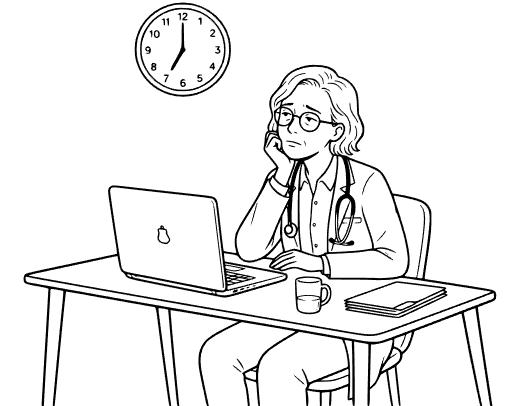
\includegraphics[width=\columnwidth]{img/escena1.jpg}
\caption{Viñeta 1: Contexto y necesidad.}
\label{fig:vineta1}
\end{figure}

\begin{figure}[H]
\centering
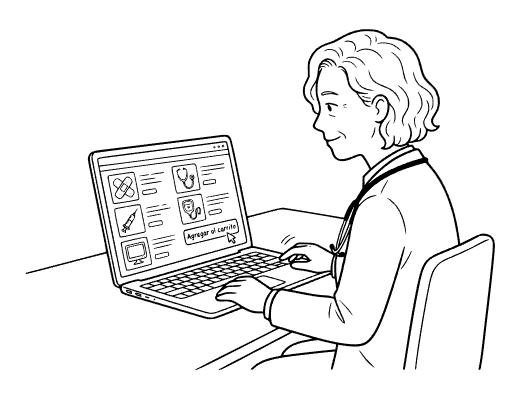
\includegraphics[width=\columnwidth]{img/escena2.jpg}
\caption{Viñeta 2: Interacción exitosa con la interfaz.}
\label{fig:vineta2}
\end{figure}

\begin{figure}[H]
\centering
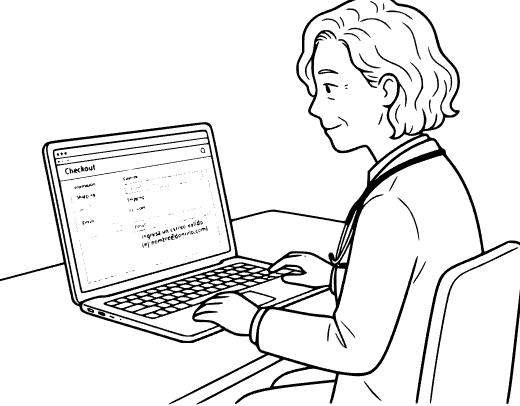
\includegraphics[width=\columnwidth]{img/escena3.jpg}
\caption{Viñeta 3: Encuentro con error orientativo.}
\label{fig:vineta3}
\end{figure}

\begin{figure}[H]
\centering
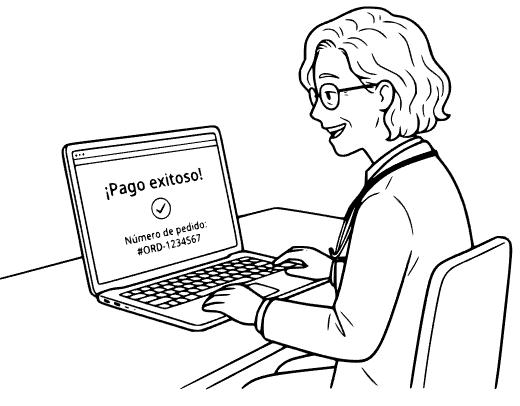
\includegraphics[width=\columnwidth]{img/escena4.jpg}
\caption{Viñeta 4: Confirmación de éxito en la transacción.}
\label{fig:vineta4}
\end{figure}

\begin{figure}[H]
\centering
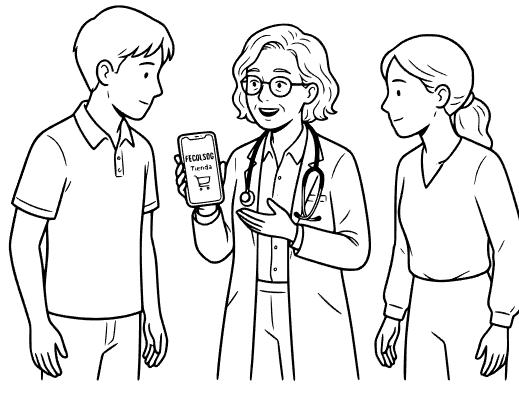
\includegraphics[width=\columnwidth]{img/escena5.jpg}
\caption{Viñeta 5: Fidelización y recomendación.}
\label{fig:vineta5}
\end{figure}

\subsection{Microcopy rediseñado para flujos críticos}

\subsubsection{Marco general del rediseño}

La Tabla~\ref{tab:problemas-soluciones} sistematiza los problemas de microcopy identificados en el diagnóstico, la heurística o criterio WCAG violado y la solución propuesta. Cada intervención sigue el principio de Yifrah \cite{ux-writing} de que el microcopy efectivo debe responder tres preguntas implícitas del usuario: ¿qué ocurrió?, ¿por qué ocurrió? y ¿qué debe hacerse ahora?

\begin{table*}[t]
\centering
\caption{Problemas de microcopy y soluciones propuestas}
\label{tab:problemas-soluciones}
\renewcommand{\arraystretch}{1.2}
\begin{tabular}{|p{3.5cm}|p{4.5cm}|p{7cm}|}
\hline
\textbf{Problema identificado} & \textbf{Heurística / Criterio WCAG violado} & \textbf{Solución propuesta} \\
\hline
Mensajes de error inexistentes o genéricos & H9 / WCAG 3.3.1 (Identificación de errores) & Mensajes específicos que indiquen qué falló, por qué y cómo corregirlo \\
\hline
Botones con etiquetas ambiguas (``Comprar'') & H5 / WCAG 2.4.6 (Encabezados y etiquetas) & Verbos de acción específicos: ``Agregar al carrito'', ``Confirmar inscripción'' \\
\hline
Campos de formulario sin etiquetas visibles & H6 / WCAG 3.3.2 (Etiquetas o instrucciones) & Etiquetas visibles vinculadas al campo mediante \texttt{for/id} \\
\hline
Ausencia de confirmaciones post-acción & H1: Visibilidad del estado del sistema & Mensajes de éxito con resumen y número de referencia \\
\hline
Lenguaje técnico en errores (``Error 503'') & H2 / WCAG 3.3.3 & Traducción a lenguaje natural con acciones concretas \\
\hline
\end{tabular}
\end{table*}

\subsubsection{Flujo de compra — Selección de producto}

\begin{table}[H]
\centering
\caption{Microcopy rediseñado: selección de producto}
\label{tab:producto}
\setlength{\tabcolsep}{3pt}
\renewcommand{\arraystretch}{1.2}
\begin{tabular}{|p{1.8cm}|p{2.2cm}|p{3cm}|}
\hline
\textbf{Elemento} & \textbf{Original} & \textbf{Rediseñado} \\
\hline
Botón principal & \malEjemplo{Comprar} & \buenEjemplo{Agregar al carrito} \\
\hline
Error: opción no seleccionada & Sin mensaje & \buenEjemplo{Seleccione una [talla/color] antes de agregar al carrito} \\
\hline
\end{tabular}
\end{table}

\subsubsection{Flujo de compra — Formulario de datos}

Los campos de formulario sin etiquetas visibles transgreden WCAG 3.3.2 y la heurística H6. El rediseño (Tabla~\ref{tab:formulario}) introduce etiquetas persistentes y mensajes de error \textit{proxémicos}, ubicados junto al campo que los origina, en cumplimiento de WCAG 3.3.1 y 3.3.3.

\begin{table}[H]
\centering
\caption{Microcopy rediseñado: formulario de datos}
\label{tab:formulario}
\setlength{\tabcolsep}{3pt}
\renewcommand{\arraystretch}{1.2}
\begin{tabular}{|p{1.8cm}|p{2.2cm}|p{3cm}|}
\hline
\textbf{Elemento} & \textbf{Original} & \textbf{Rediseñado} \\
\hline
Campo de identificación & Sin etiqueta & \buenEjemplo{Etiqueta: ``Número de identificación'' + placeholder colombiano} \\
\hline
Error: campo vacío & ``Campo obligatorio'' (al final) & \buenEjemplo{``El número de identificación es obligatorio''} (junto al campo) \\
\hline
Error: formato de correo & ``Correo errado'' & \buenEjemplo{``Ingrese un correo válido (ej: nombre@dominio.com)''} \\
\hline
\end{tabular}
\end{table}

\subsubsection{Flujo de compra — Proceso de pago}

\begin{table}[H]
\centering
\caption{Microcopy rediseñado: proceso de pago}
\label{tab:pago}
\setlength{\tabcolsep}{3pt}
\renewcommand{\arraystretch}{1.2}
\begin{tabular}{|p{1.8cm}|p{2.2cm}|p{3cm}|}
\hline
\textbf{Elemento} & \textbf{Original} & \textbf{Rediseñado} \\
\hline
Procesando pago & Sin indicador & \buenEjemplo{``Se está procesando el pago. No cierre esta ventana.''} \\
\hline
Pago exitoso & ``Transacción completada'' & \buenEjemplo{``¡Pago realizado! Su pedido \#12345 ha sido confirmado.''} \\
\hline
Pago fallido & ``Error al procesar'' & \buenEjemplo{``No fue posible procesar el pago. ¿Desea intentar con otra tarjeta?''} \\
\hline
\end{tabular}
\end{table}

\subsubsection{Flujo de búsqueda y navegación}

\begin{table}[H]
\centering
\caption{Microcopy rediseñado: búsqueda}
\label{tab:busqueda}
\setlength{\tabcolsep}{3pt}
\renewcommand{\arraystretch}{1.2}
\begin{tabular}{|p{1.8cm}|p{2.2cm}|p{3cm}|}
\hline
\textbf{Elemento} & \textbf{Original} & \textbf{Rediseñado} \\
\hline
Sin resultados & No disponible & \buenEjemplo{``No se encontraron productos para `bata azul'. Pruebe con: `bata', `uniforme'.''} \\
\hline
Carga de resultados & Sin indicador & \buenEjemplo{``Buscando productos...''} + indicador de progreso \\
\hline
\end{tabular}
\end{table}

\subsubsection{Flujo de inscripción a eventos}

\begin{table}[H]
\centering
\caption{Microcopy rediseñado: inscripción a eventos}
\label{tab:eventos}
\setlength{\tabcolsep}{3pt}
\renewcommand{\arraystretch}{1.2}
\begin{tabular}{|p{1.8cm}|p{2.2cm}|p{3cm}|}
\hline
\textbf{Elemento} & \textbf{Original} & \textbf{Rediseñado} \\
\hline
Inscripción exitosa & ``Inscripción registrada'' & \buenEjemplo{``Se ha inscrito al `Congreso 2026'. Revise su correo para confirmar.''} \\
\hline
Fecha límite cercana & Sin advertencia & \buenEjemplo{``La inscripción cierra en 3 días. Regístrese ahora.''} \\
\hline
\end{tabular}
\end{table}

\subsubsection{Mensajes de error generales}

\begin{table}[H]
\centering
\caption{Mensajes de error generales rediseñados}
\label{tab:errores-generales}
\setlength{\tabcolsep}{3pt}
\renewcommand{\arraystretch}{1.2}
\begin{tabular}{|p{1.8cm}|p{2.2cm}|p{3cm}|}
\hline
\textbf{Tipo} & \textbf{Original} & \textbf{Rediseñado} \\
\hline
Error de servidor & ``Error 503'' & \buenEjemplo{``No fue posible conectar. Verifique su conexión e intente nuevamente.''} \\
\hline
Página no encontrada & ``Error 404'' & \buenEjemplo{``La página no existe. Puede volver al inicio o usar el buscador.''} \\
\hline
\end{tabular}
\end{table}

% ─────────────────────────────────────────────────────────────────────────────
\section{Implementación Técnica — Entregable 3}
% ─────────────────────────────────────────────────────────────────────────────

\subsection{Arquitectura y pila tecnológica}

La implementación se construyó sobre Astro~5 \cite{astro-docs}, un framework de generación de sitios estáticos orientado al rendimiento y a la accesibilidad. La arquitectura \textit{islands} de Astro permite que los componentes interactivos —carrito, favoritos, notificaciones— sean hidratados selectivamente en el cliente mediante React~19, mientras que el resto del contenido se sirve como HTML estático \cite{astro-docs}. Esta estrategia minimiza el JavaScript enviado al navegador y favorece la compatibilidad con tecnologías de asistencia.

El sistema de estilos emplea Tailwind CSS~v4 en su modo de configuración CSS-first \cite{tailwind-docs}, lo que elimina la necesidad de un fichero de configuración JavaScript y reduce la fricción en el mantenimiento del sistema de diseño. DaisyUI~v5 \cite{daisyui-docs} provee un conjunto de componentes semánticamente correctos —botones, formularios, menús desplegables— que implementan por defecto los patrones ARIA recomendados por WAI-ARIA 1.2 \cite{wai-aria}.

El sistema de gestión de estado se implementa mediante \textit{nanostores} con persistencia en \texttt{localStorage}, un enfoque isomórfico compatible con la arquitectura SSG que preserva el estado del carrito entre sesiones sin requerir autenticación de servidor.

\subsection{Sistema de diseño y tema de accesibilidad}

Se definió un tema institucional denominado \texttt{fecolsog} mediante variables de color en formato OKLCH, el espacio de color perceptualmente uniforme recomendado por el nivel 4 de CSS \cite{css-color-4}. El color primario (\texttt{oklch(40\% 0.157 247)}, correspondiente aproximadamente a \#004F9F) sobre fondo blanco (\texttt{oklch(100\% 0 0)}) produce una relación de contraste de 8,6:1, que supera el umbral de 7:1 exigido por el nivel AAA de WCAG 2.1 \cite{wcag-2018} para texto normal, y el de 4,5:1 del nivel AA, que era el criterio incumplido en la versión original de la tienda.

La Tabla~\ref{tab:contraste} compara los valores de contraste antes y después del rediseño para los pares cromáticos críticos de la interfaz.

\begin{table}[H]
\centering
\caption{Comparación de relaciones de contraste cromático}
\label{tab:contraste}
\setlength{\tabcolsep}{3pt}
\renewcommand{\arraystretch}{1.2}
\begin{tabular}{|p{2.5cm}|p{1.5cm}|p{1.5cm}|p{1.5cm}|}
\hline
\textbf{Par cromático} & \textbf{Antes} & \textbf{Después} & \textbf{Nivel} \\
\hline
Texto primario / fondo & 1,61:1 & 8,6:1 & AAA \\
\hline
Texto navegación / fondo primario & 2,3:1 & 12,1:1 & AAA \\
\hline
Texto body / fondo base & 4,1:1 & 14,7:1 & AAA \\
\hline
Texto secundario / fondo & 3,8:1 & 5,2:1 & AA \\
\hline
\end{tabular}
\end{table}

\subsection{Criterios WCAG 2.1 implementados}

La Tabla~\ref{tab:wcag-implementados} documenta los criterios de éxito WCAG 2.1 que presentaban violaciones en el diagnóstico y el mecanismo técnico implementado para su corrección. La columna ``Nivel'' indica el nivel de conformidad alcanzado: A (mínimo), AA (estándar de referencia) o AAA (nivel óptimo).

\begin{table*}[t]
\centering
\caption{Criterios WCAG 2.1 corregidos en la implementación}
\label{tab:wcag-implementados}
\renewcommand{\arraystretch}{1.2}
\begin{tabular}{|p{1.2cm}|p{3.5cm}|p{6cm}|p{1.5cm}|p{1.5cm}|}
\hline
\textbf{Criterio} & \textbf{Descripción} & \textbf{Implementación} & \textbf{Nivel orig.} & \textbf{Nivel final} \\
\hline
1.3.1 & Información y relaciones & Estructura semántica con \texttt{<nav aria-label>}, \texttt{<main id>}, \texttt{<article>}, \texttt{<section aria-label>}; breadcrumbs con Schema.org BreadcrumbList y \texttt{aria\-current="page"} & Falla & A \\
\hline
1.3.5 & Identificar el propósito de entrada & Atributos \texttt{autocomplete} en todos los campos de formulario (given-name, family-name, email, tel) & Falla & AA \\
\hline
1.4.3 & Contraste mínimo & Tema OKLCH con ratio 8,6:1 para texto sobre fondo & Falla (1,61:1) & AAA \\
\hline
1.4.4 & Cambio de tamaño del texto & \texttt{meta viewport} con \texttt{initial-scale=1} sin \texttt{user-scalable=no}; tamaños de fuente en \texttt{rem} & Falla & AA \\
\hline
2.1.1 & Teclado & Todos los elementos interactivos alcanzables y operables por teclado & Falla parcial & A \\
\hline
2.4.1 & Evitar bloques & Enlace ``Ir al contenido principal'' oculto visualmente, visible al recibir foco; \texttt{id="main-content"} en \texttt{<main>} & Falla & A \\
\hline
2.4.7 & Foco visible & \texttt{:focus-visible} global con anillo azul de 3px y offset de 3px & Falla & AA \\
\hline
3.1.1 & Idioma de la página & \texttt{<html lang="es">} & Falla & A \\
\hline
3.3.2 & Etiquetas o instrucciones & Etiquetas \texttt{<label for>} visibles y persistentes en todos los campos; texto de ayuda bajo los campos complejos & Falla & A \\
\hline
\end{tabular}
\end{table*}

\subsection{Componentes de navegación accesible}

\subsubsection{Enlace de salto de navegación}

Se implementó un enlace de omisión (\textit{skip link}) conforme al patrón recomendado por WebAIM \cite{webaim-skip}: visualmente oculto mediante la clase utilitaria \texttt{sr-only} de Tailwind, pero presentado visualmente al recibir foco de teclado mediante \texttt{focus:not-sr-only}. El destino del enlace es el elemento \texttt{main} con \texttt{id="main-content"} y \texttt{tabindex="-1"}, que garantiza que el foco de teclado se desplace efectivamente al inicio del contenido principal sin requerir JavaScript.

\subsubsection{Breadcrumbs semánticos}

El componente de breadcrumbs fue reescrito con una estructura \texttt{nav} con \texttt{aria-label} que contiene una lista ordenada \texttt{ol} con microdata Schema.org \texttt{BreadcrumbList}. El ítem activo (página actual) lleva el atributo \texttt{aria-current="page"}, lo que permite a los lectores de pantalla anunciar correctamente la posición del usuario dentro de la jerarquía del sitio. Esta implementación satisface simultáneamente el criterio WCAG 1.3.1 (Información y relaciones) y las recomendaciones de Google para datos estructurados \cite{google-structured-data}.

\subsection{Catálogo de productos y arquitectura de contenido}

La versión original de la tienda FECOLSOG ofrecía un catálogo de cuatro productos sin estructura de categorías, imágenes de baja calidad y descripciones genéricas de una línea. El rediseño implementó una arquitectura de contenido de dos niveles (categoría / producto) con 33 productos distribuidos en seis categorías especializadas (Tabla~\ref{tab:catalogo}), coherentes con las líneas de negocio reales de la federación identificadas en el diagnóstico.

\begin{table}[H]
\centering
\caption{Arquitectura del catálogo rediseñado}
\label{tab:catalogo}
\setlength{\tabcolsep}{3pt}
\renewcommand{\arraystretch}{1.2}
\begin{tabular}{|p{2.5cm}|p{1cm}|p{4cm}|}
\hline
\textbf{Categoría} & \textbf{Prods.} & \textbf{Ejemplos representativos} \\
\hline
Indumentaria & 5 & Bata médica, Traje antifluido \\
\hline
Insumos Médicos & 3 & Guantes de examinación, Mascarilla N95 \\
\hline
Dispositivos & 3 & Tensiómetro digital, Oxímetro de pulso \\
\hline
Educación & 9 & Guía clínica GO 2025, Curso de colposcopía online \\
\hline
Artículos & 11 & Polo corporativo, Agenda médica 2026 \\
\hline
Congresos & 2 & Entrada Congreso Nacional 2025 \\
\hline
\end{tabular}
\end{table}

\subsection{Contenido editorial: blog médico}

Se incorporó un módulo editorial con ocho artículos de blog redactados en tono profesional e impersonal, firmados por especialistas ficticios con formación en las subespecialidades representadas por FECOLSOG. Los temas cubren: manejo de endometriosis, atención prenatal de bajo riesgo, anticoncepción moderna, tamizaje de cáncer de cuello uterino, menopausia y salud cardiovascular, ultrasonido en el primer trimestre y hemorragia posparto. Este contenido cumple una función dual: proveer valor informativo al profesional de la salud y contribuir al posicionamiento orgánico (SEO) de la plataforma mediante contenido estructurado con etiquetas semánticas HTML5.

\subsection{Páginas de soporte informativo}

La versión original carecía de páginas de soporte independientes. El rediseño incorporó tres páginas de política institucional:

\begin{itemize}
    \item \textbf{Preguntas frecuentes (\texttt{/faq}):} 18 preguntas organizadas en cinco secciones temáticas implementadas mediante el elemento nativo \texttt{<details>}/\texttt{<summary>} de HTML5, que provee comportamiento de acordeón sin JavaScript y con semántica ARIA nativa.
    \item \textbf{Política de envíos (\texttt{/envios}):} tres zonas de cobertura con tiempos y condiciones, proceso de despacho visualizado como línea de tiempo.
    \item \textbf{Política de devoluciones (\texttt{/devoluciones}):} tablas de casos por tipo de producto con indicadores visuales $\checkmark$/$\times$, enmarcadas en la Ley 1480 de 2011 (Estatuto del Consumidor colombiano).
\end{itemize}

\subsection{Comparación visual antes/después}

Las Figuras~\ref{fig:before-home} y~\ref{fig:after-home} ilustran el estado de la página de inicio antes y después del rediseño. La versión original presenta una navegación horizontal con separadores de texto, ausencia de jerarquía visual, fondo blanco sin estructura y productos listados sin contexto visual. La versión rediseñada incorpora una barra de anuncios contextual, navegación por categorías con menús desplegables, un hero con carrusel de imágenes de alta resolución y una sección de categorías con imágenes representativas.

\begin{figure}[H]
\centering
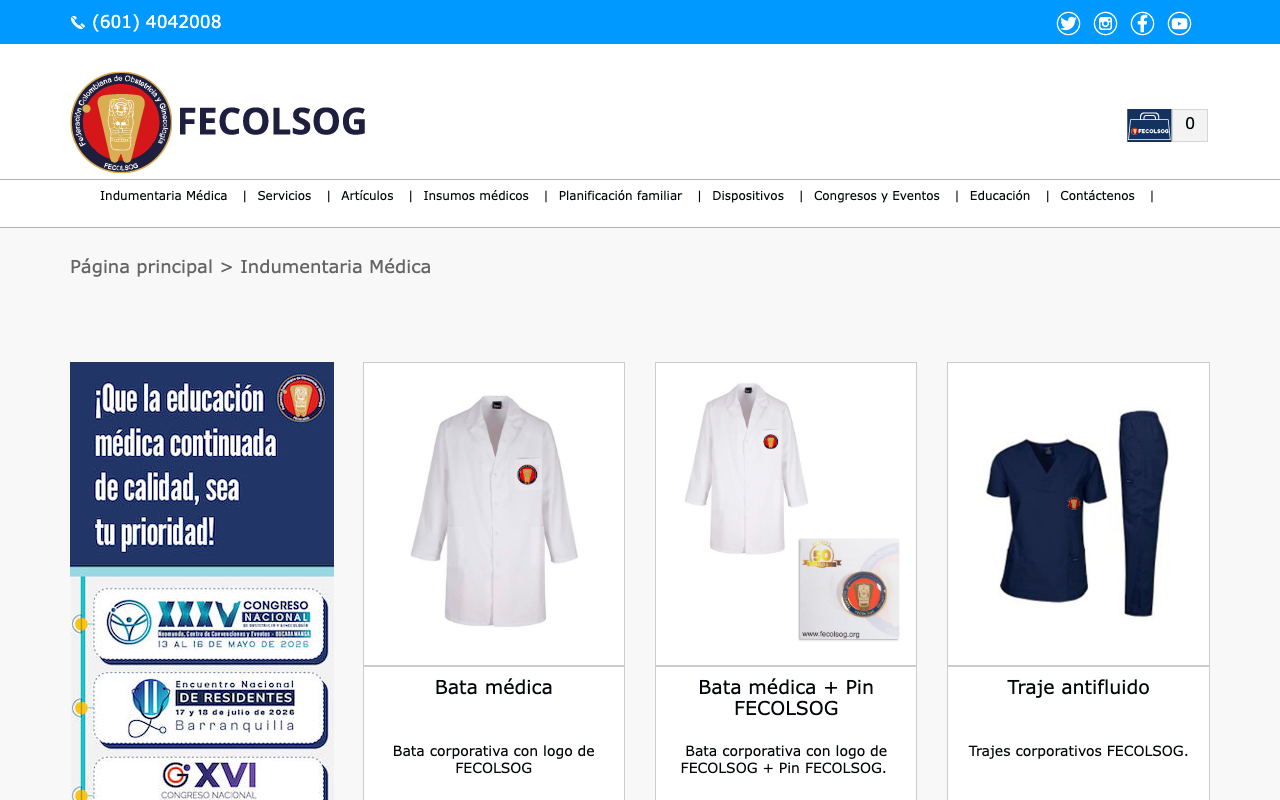
\includegraphics[width=\columnwidth]{img/before-home.png}
\caption{Página de inicio original de la tienda FECOLSOG. Se observa navegación plana, ausencia de jerarquía visual y catálogo sin estructura de categorías.}
\label{fig:before-home}
\end{figure}

\begin{figure}[H]
\centering
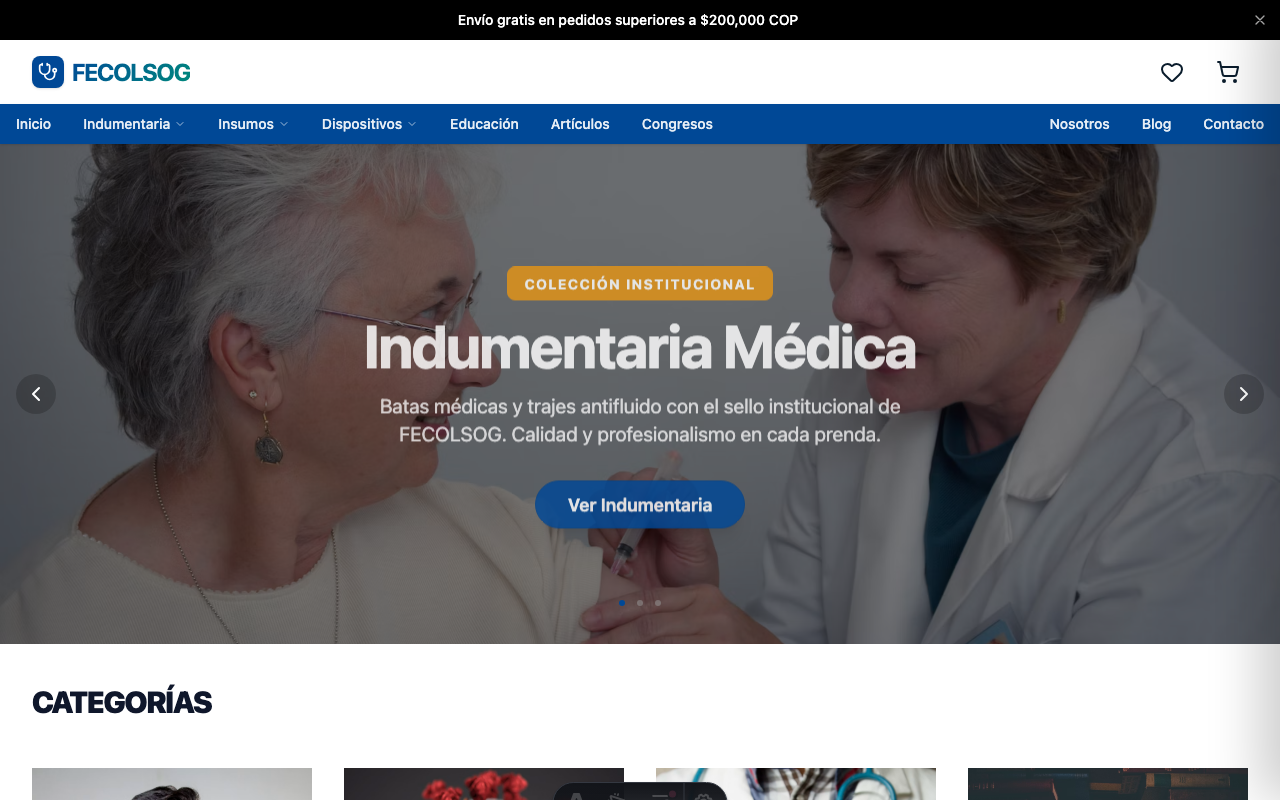
\includegraphics[width=\columnwidth]{img/after-home.png}
\caption{Página de inicio rediseñada. Se incorporan barra de anuncios accesible, navegación categorizada con menú desplegable, hero con imagen contextual y sección de categorías.}
\label{fig:after-home}
\end{figure}

Las Figuras~\ref{fig:after-product} y~\ref{fig:after-checkout} documentan dos flujos críticos en la versión rediseñada. La página de producto (Fig.~\ref{fig:after-product}) presenta el precio en moneda local (COP con formato colombiano), el estado de inventario, especificaciones técnicas y botones con etiquetas de acción específicas. El formulario de checkout (Fig.~\ref{fig:after-checkout}) implementa los campos con etiquetas visibles, \textit{placeholders} localizados para Colombia, secciones numeradas que comunican el progreso del proceso y un resumen lateral del pedido.

\begin{figure}[H]
\centering
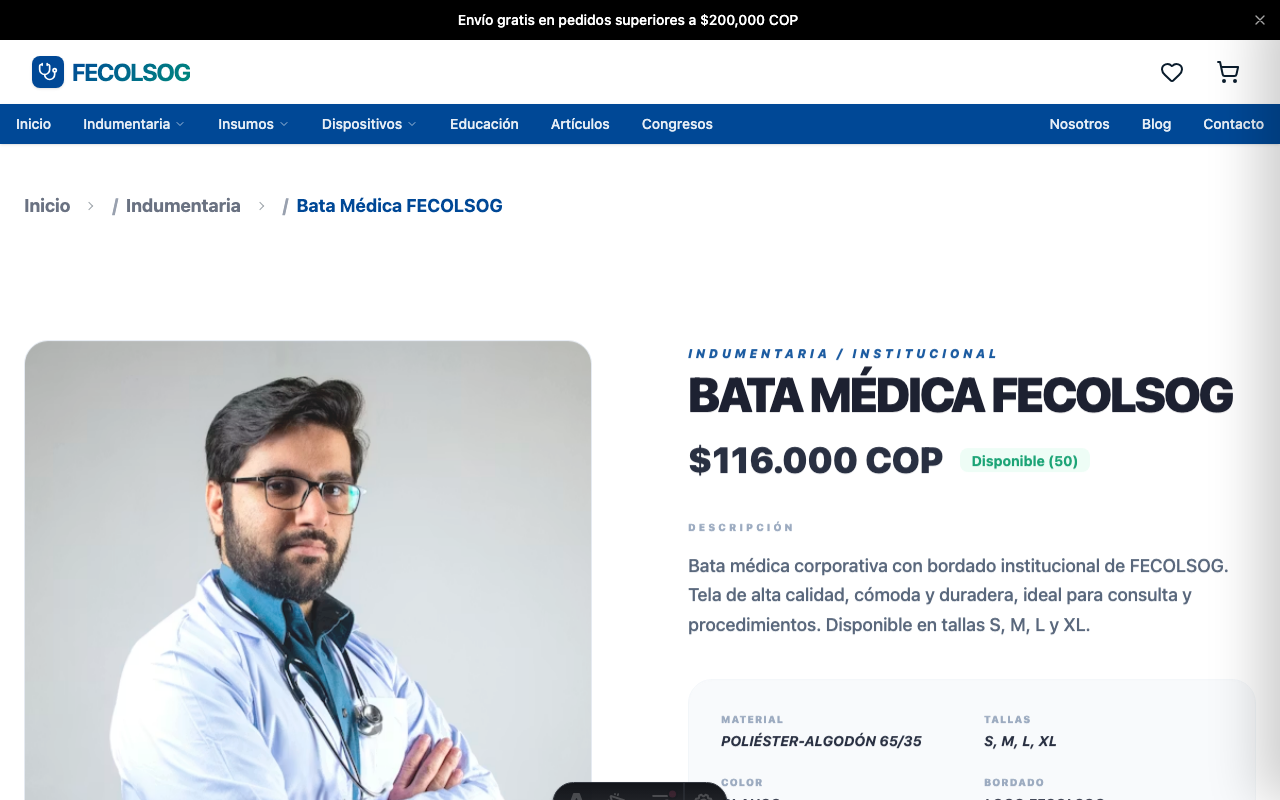
\includegraphics[width=\columnwidth]{img/after-product.png}
\caption{Página de producto rediseñada. Precio en COP, estado de inventario, especificaciones técnicas y botones con etiquetas de acción específicas.}
\label{fig:after-product}
\end{figure}

\begin{figure}[H]
\centering
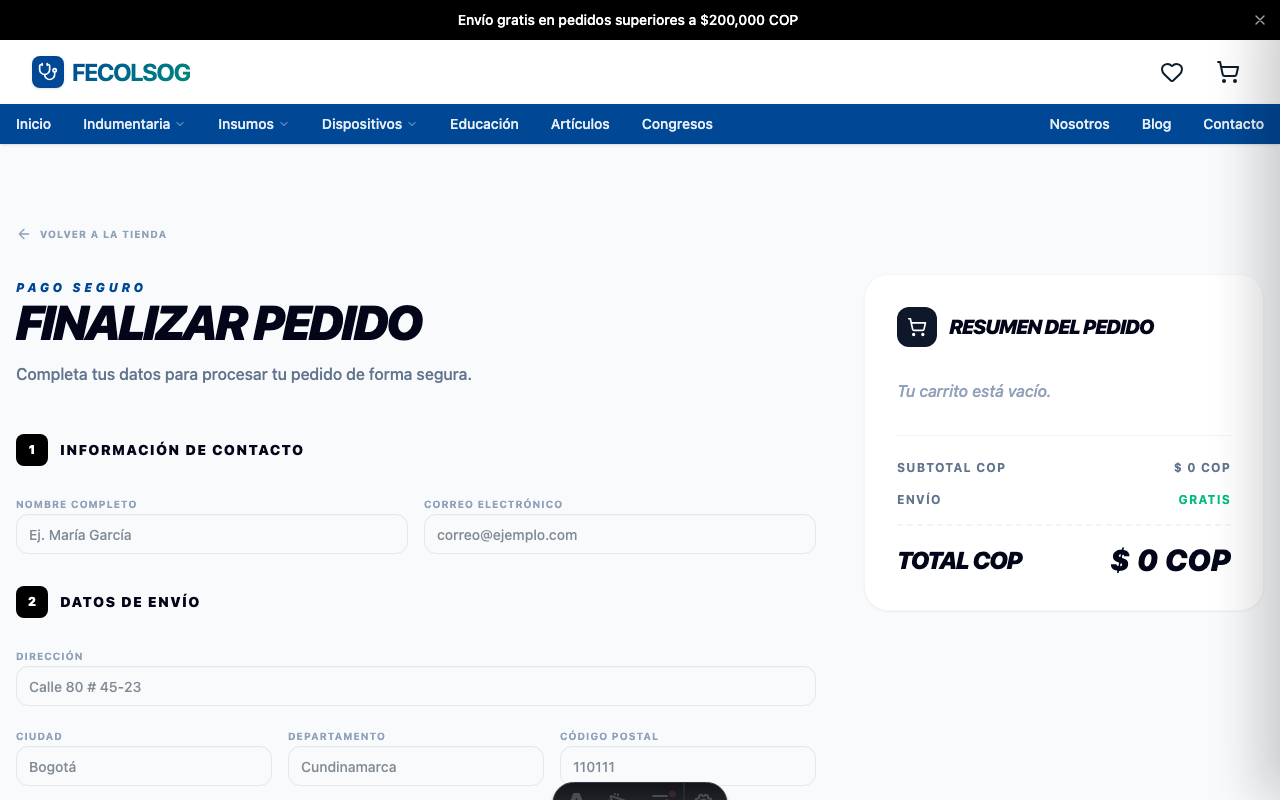
\includegraphics[width=\columnwidth]{img/after-checkout.png}
\caption{Formulario de checkout rediseñado. Etiquetas visibles, secciones numeradas, placeholders localizados y resumen del pedido en tiempo real.}
\label{fig:after-checkout}
\end{figure}

Las Figuras~\ref{fig:before-404} y~\ref{fig:after-404} ilustran uno de los casos de microcopy más críticos: la página de error 404. La versión original presenta la respuesta de error genérica del servidor web (IIS) en inglés, sin navegación de la marca, sin contexto y sin ninguna acción orientativa para el usuario. El mensaje ``404 - File or directory not found. The resource you are looking for might have been removed, had its name changed, or is temporarily unavailable'' viola simultáneamente la heurística H2 de Nielsen (Coincidencia entre el sistema y el mundo real) —al emplear lenguaje técnico del sistema— y la heurística H9 (Ayudar a los usuarios a reconocer, diagnosticar y recuperarse de errores) —al no proveer ninguna ruta de recuperación—. Adicionalmente, la ausencia de estructura HTML y de etiqueta \texttt{lang} constituye una violación de los criterios WCAG 3.1.1 y 1.3.1.

La versión rediseñada mantiene el contexto institucional completo (barra de anuncios, navegación categorizada y marca FECOLSOG), reemplaza el código técnico por el mensaje ``Página no encontrada :/'' en español e incorpora una descripción empática con una acción de recuperación explícita: el botón ``Volver al inicio'', en cumplimiento de las heurísticas H2, H9 y el criterio WCAG 3.3.3.

\begin{figure}[H]
\centering
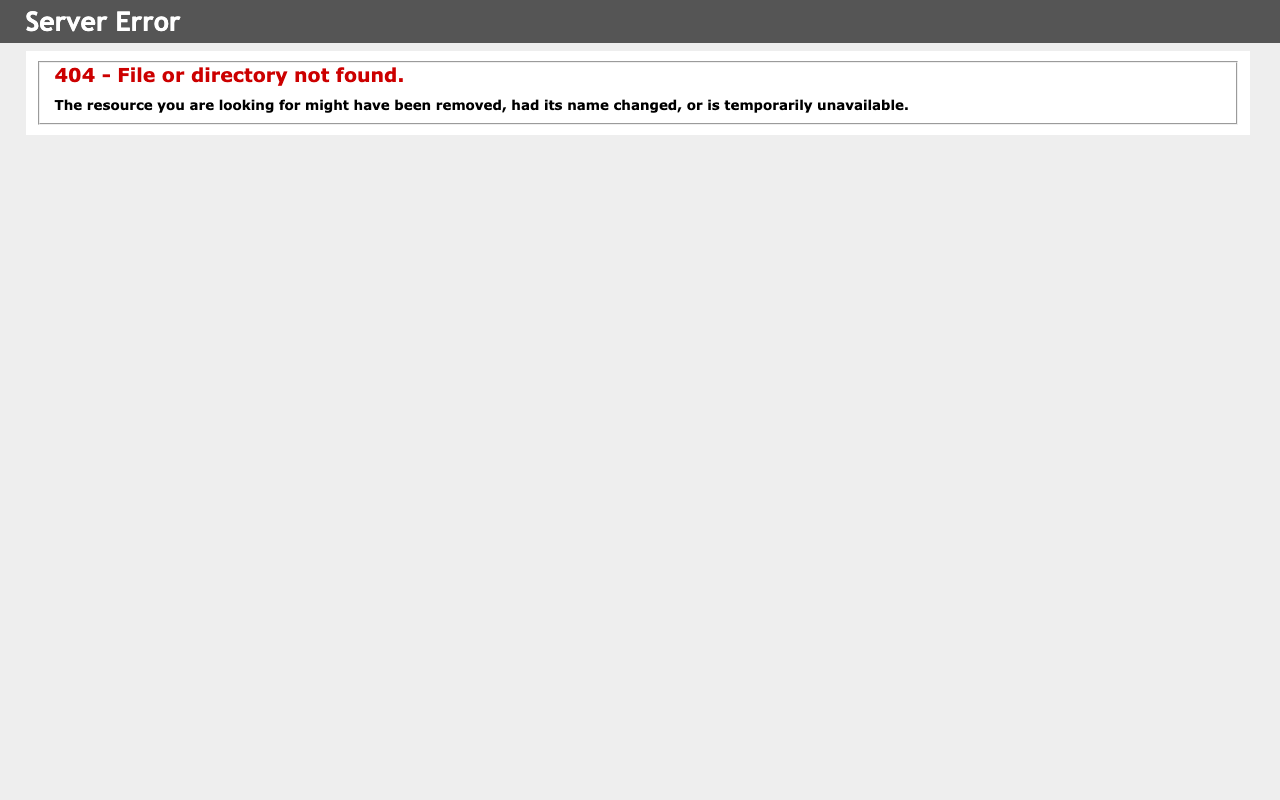
\includegraphics[width=\columnwidth]{img/before-404.png}
\caption{Página de error 404 original. Respuesta genérica del servidor en inglés, sin navegación institucional ni acciones de recuperación. Viola H2, H9 (Nielsen) y WCAG 3.1.1, 1.3.1.}
\label{fig:before-404}
\end{figure}

\begin{figure}[H]
\centering
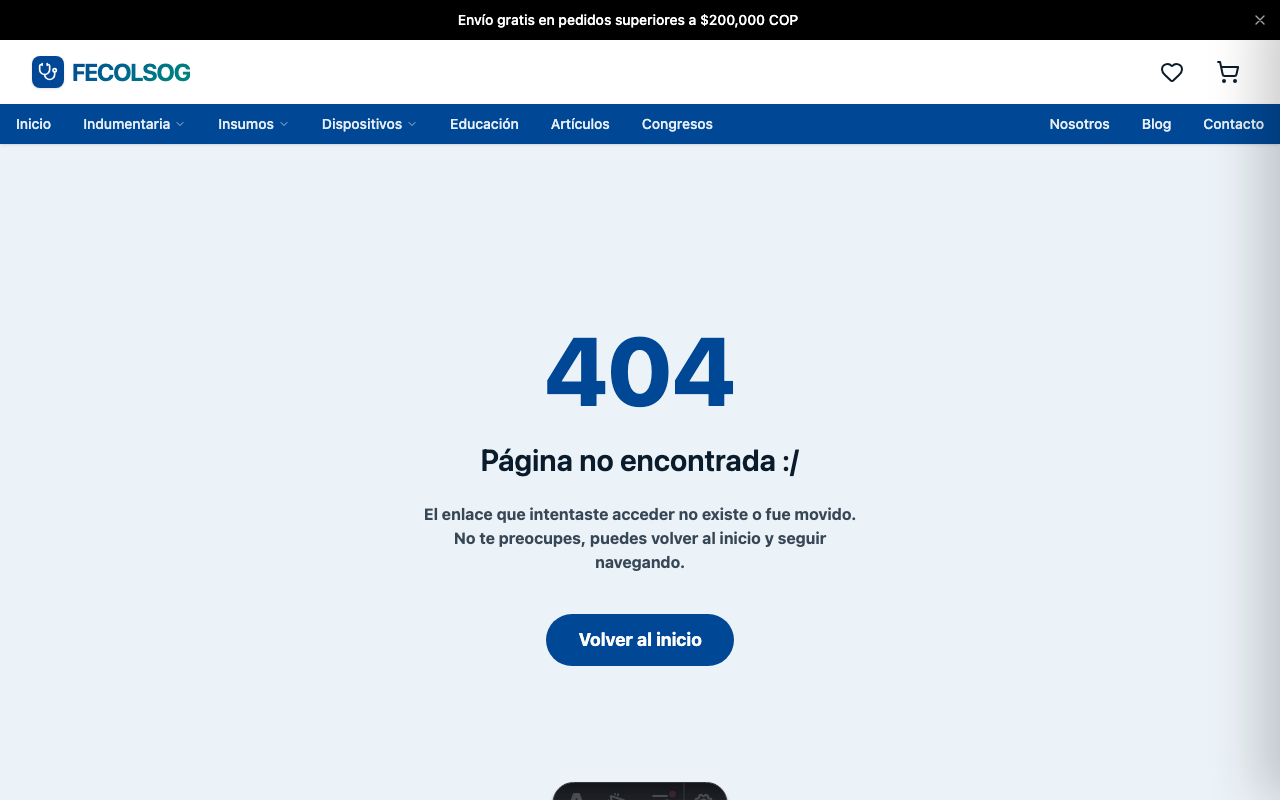
\includegraphics[width=\columnwidth]{img/after-404.png}
\caption{Página 404 rediseñada. Mensaje en español con tono empático, navegación institucional completa y botón de acción ``Volver al inicio''. Cumple H2, H9 (Nielsen) y WCAG 3.3.3.}
\label{fig:after-404}
\end{figure}

% ─────────────────────────────────────────────────────────────────────────────
\section{Conclusión}
% ─────────────────────────────────────────────────────────────────────────────

El trabajo presentado desarrolló un rediseño integral de la tienda en línea de FECOLSOG abordando de forma articulada las dimensiones de contenido e interfaz.

Desde la perspectiva del contenido (Entregable~2), la definición de voz y tono —profesional, cercana y confiable, con variaciones contextuales fundamentadas en las heurísticas de Nielsen \cite{nielsen-1994}— provee una guía comunicativa coherente aplicable a todos los puntos de contacto. El arco narrativo de la Dra. María Restrepo, construido sobre el modelo de Quesenbery y Brooks \cite{storytelling-ux}, identifica los momentos de mayor riesgo de abandono y los factores de fidelización como criterios concretos de diseño. El microcopy rediseñado transforma mensajes ambiguos o ausentes en orientaciones claras, específicas y accionables que cumplen los criterios WCAG 2.1 \cite{wcag-2018}.

Desde la perspectiva de la implementación (Entregable~3), se materializaron nueve criterios de éxito WCAG 2.1 que presentaban violaciones en el diagnóstico inicial. Los resultados más significativos comprenden: la corrección de la relación de contraste cromático de 1,61:1 a 8,6:1 —superando el nivel AAA—, la incorporación del enlace de salto de navegación para usuarios de teclado y lectores de pantalla, la implementación de etiquetas semánticas y \texttt{aria-label} en todos los elementos de navegación, y la adición del atributo \texttt{autocomplete} en los formularios de contacto y checkout. Paralelamente, el catálogo se expandió de 4 a 33 productos en seis categorías especializadas, el sitio incorporó contenido editorial médico de valor para el profesional de la salud y se crearon páginas de política institucional ausentes en la versión original.

Los tres componentes del Entregable~2 y las mejoras del Entregable~3 convergen en un objetivo común: reducir la fricción cognitiva de un usuario experto en su campo pero con baja tolerancia a interfaces mal diseñadas, incrementando así la probabilidad de conversión y fidelización en una plataforma de servicios académicos especializados.

% ─────────────────────────────────────────────────────────────────────────────
\begin{thebibliography}{99}
% ─────────────────────────────────────────────────────────────────────────────

\bibitem{nielsen-1994}
J. Nielsen, \textit{Usability Engineering}. San Francisco, CA, USA: Morgan Kaufmann, 1994.

\bibitem{wcag-2018}
B. Caldwell y M. Cooper, ``Web Content Accessibility Guidelines (WCAG) 2.1,'' W3C Recommendation, Jun. 2018. [En línea]. Disponible: \url{https://www.w3.org/TR/WCAG21/}

\bibitem{nng-voice}
K. Moran, ``Voice and Tone: How to Define and Document Your Brand's Personality,'' Nielsen Norman Group, 2020. [En línea]. Disponible: \url{https://www.nngroup.com/articles/voice-tone/}

\bibitem{storytelling-ux}
A. Quesenbery y K. Brooks, \textit{Storytelling for User Experience: Crafting Stories for Better Design}. Brooklyn, NY, USA: Rosenfeld Media, 2010.

\bibitem{ux-writing}
K. Yifrah, \textit{Microcopy: The Complete Guide}. 2019.

\bibitem{sitio-web}
FECOLSOG, ``Tienda en línea,'' Federación Colombiana de Obstetricia y Ginecología. [En línea]. Disponible: \url{https://tiendaonline.fecolsog.org}

\bibitem{lighthouse}
Google, ``Lighthouse: Automated auditing, performance metrics, and best practices,'' Google Chrome for Developers, 2024. [En línea]. Disponible: \url{https://developer.chrome.com/docs/lighthouse/}

\bibitem{astro-docs}
The Astro Technology Company, ``Astro Documentation,'' 2024. [En línea]. Disponible: \url{https://docs.astro.build}

\bibitem{tailwind-docs}
Tailwind Labs, ``Tailwind CSS Documentation,'' 2024. [En línea]. Disponible: \url{https://tailwindcss.com/docs}

\bibitem{daisyui-docs}
Pouya Saadeghi, ``DaisyUI — Tailwind CSS Components,'' 2024. [En línea]. Disponible: \url{https://daisyui.com/docs}

\bibitem{wai-aria}
J. Craig y M. Cooper, ``Accessible Rich Internet Applications (WAI-ARIA) 1.2,'' W3C Recommendation, Jun. 2023. [En línea]. Disponible: \url{https://www.w3.org/TR/wai-aria-1.2/}

\bibitem{css-color-4}
C. Lilley \textit{et al.}, ``CSS Color Module Level 4,'' W3C Candidate Recommendation, Feb. 2024. [En línea]. Disponible: \url{https://www.w3.org/TR/css-color-4/}

\bibitem{webaim-skip}
WebAIM, ``Skip Navigation Links,'' WebAIM: Web Accessibility In Mind, 2023. [En línea]. Disponible: \url{https://webaim.org/techniques/skipnav/}

\bibitem{web-vitals}
P. LePage y S. McGrath, ``Web Vitals,'' web.dev, Google, 2024. [En línea]. Disponible: \url{https://web.dev/articles/vitals}

\bibitem{google-structured-data}
Google, ``Breadcrumb (BreadcrumbList),'' Google Search Central Documentation, 2024. [En línea]. Disponible: \url{https://developers.google.com/search/docs/appearance/structured-data/breadcrumb}

\end{thebibliography}

\end{document}
